\documentclass[12pt]{article}
\usepackage[utf8]{inputenc}
\usepackage[brazilian]{babel}
\usepackage{geometry}
\geometry{a4paper, total={170mm,250mm}, left=25mm, right=25mm, top=25mm}
\usepackage{graphicx}
\usepackage{titling}
\usepackage{float}
\usepackage{amsmath}

\title{Trabalho 1 - MEC2403 (Otimização)}
\author{Kleyton da Costa (2312730)}
\date{\today}
 
\usepackage{fancyhdr}
\fancypagestyle{plain}{%  the preset of fancyhdr 
    \fancyhf{} % clear all header and footer fields
    %\fancyfoot[R]{\includegraphics[width=3cm]{di.png}}
    \fancyfoot[L]{\today}
    \fancyhead[L]{Trabalho 1}
    \fancyhead[R]{\theauthor}
}
\makeatletter
\def\@maketitle{%
  \newpage
  \null
  \vskip 1em%
  \begin{center}%
  \let \footnote \thanks
    {\LARGE \@title \par}%
    \vskip 1em%
    %{\large \@date}%
  \end{center}%
  \par
  \vskip 1em}
\makeatother

\begin{document}

\maketitle

\noindent\begin{tabular}{@{}ll}
    Aluno & \theauthor \\
    Professor &  Ivan Menezes (MEC/PUC-Rio) \\
    Data & \today
\end{tabular}


\section*{Questão 1}

\paragraph*{Letra (a)}

\begin{equation}
  f(x_{1}, x{2})= x_{1}^{2}-3x_{1}x_{2}+4x_{2}^{2}+x_{1}-x_{2}
\end{equation}

\noindent pontos iniciais $x_{0} =\{2,2\}^{t}$ e $x_{0}=\{-1,-3\}^{t}$

\begin{figure}[H]
  \centering
  \caption{Ponto Inicial: [2, 2]}
  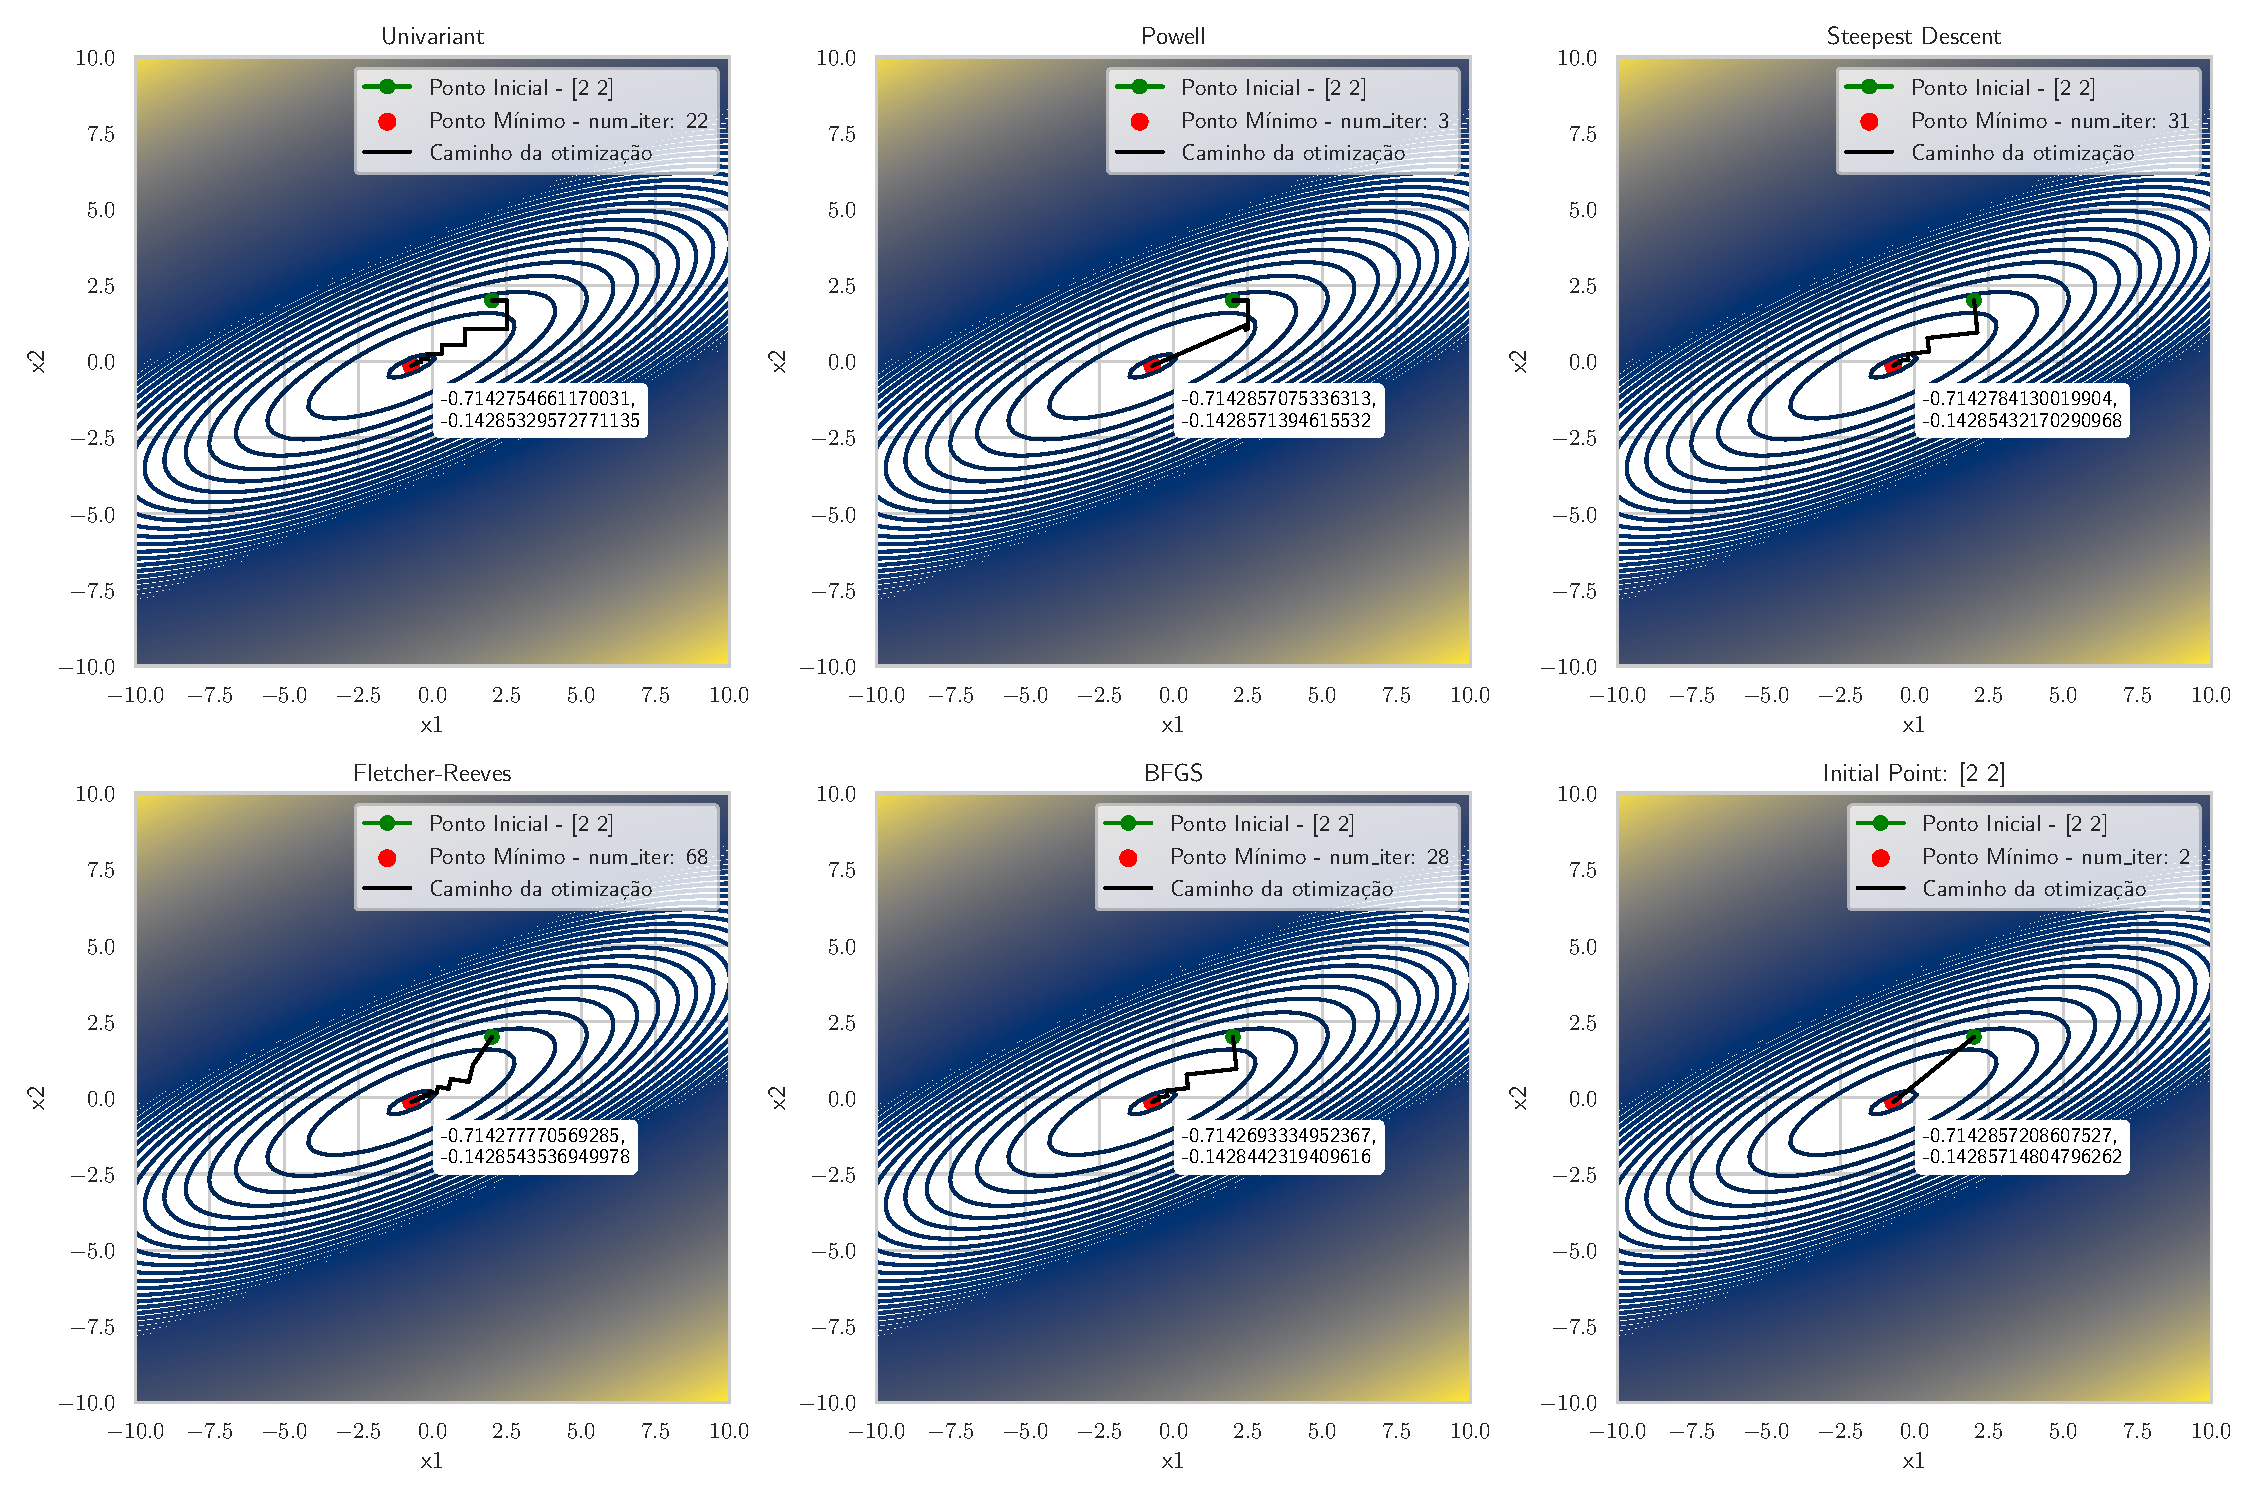
\includegraphics[scale=0.4]{img/questao_1a_[2 2].pdf}
\end{figure}

\begin{figure}[H]
  \centering
  \caption{Ponto Inicial: [-1, -3]}
  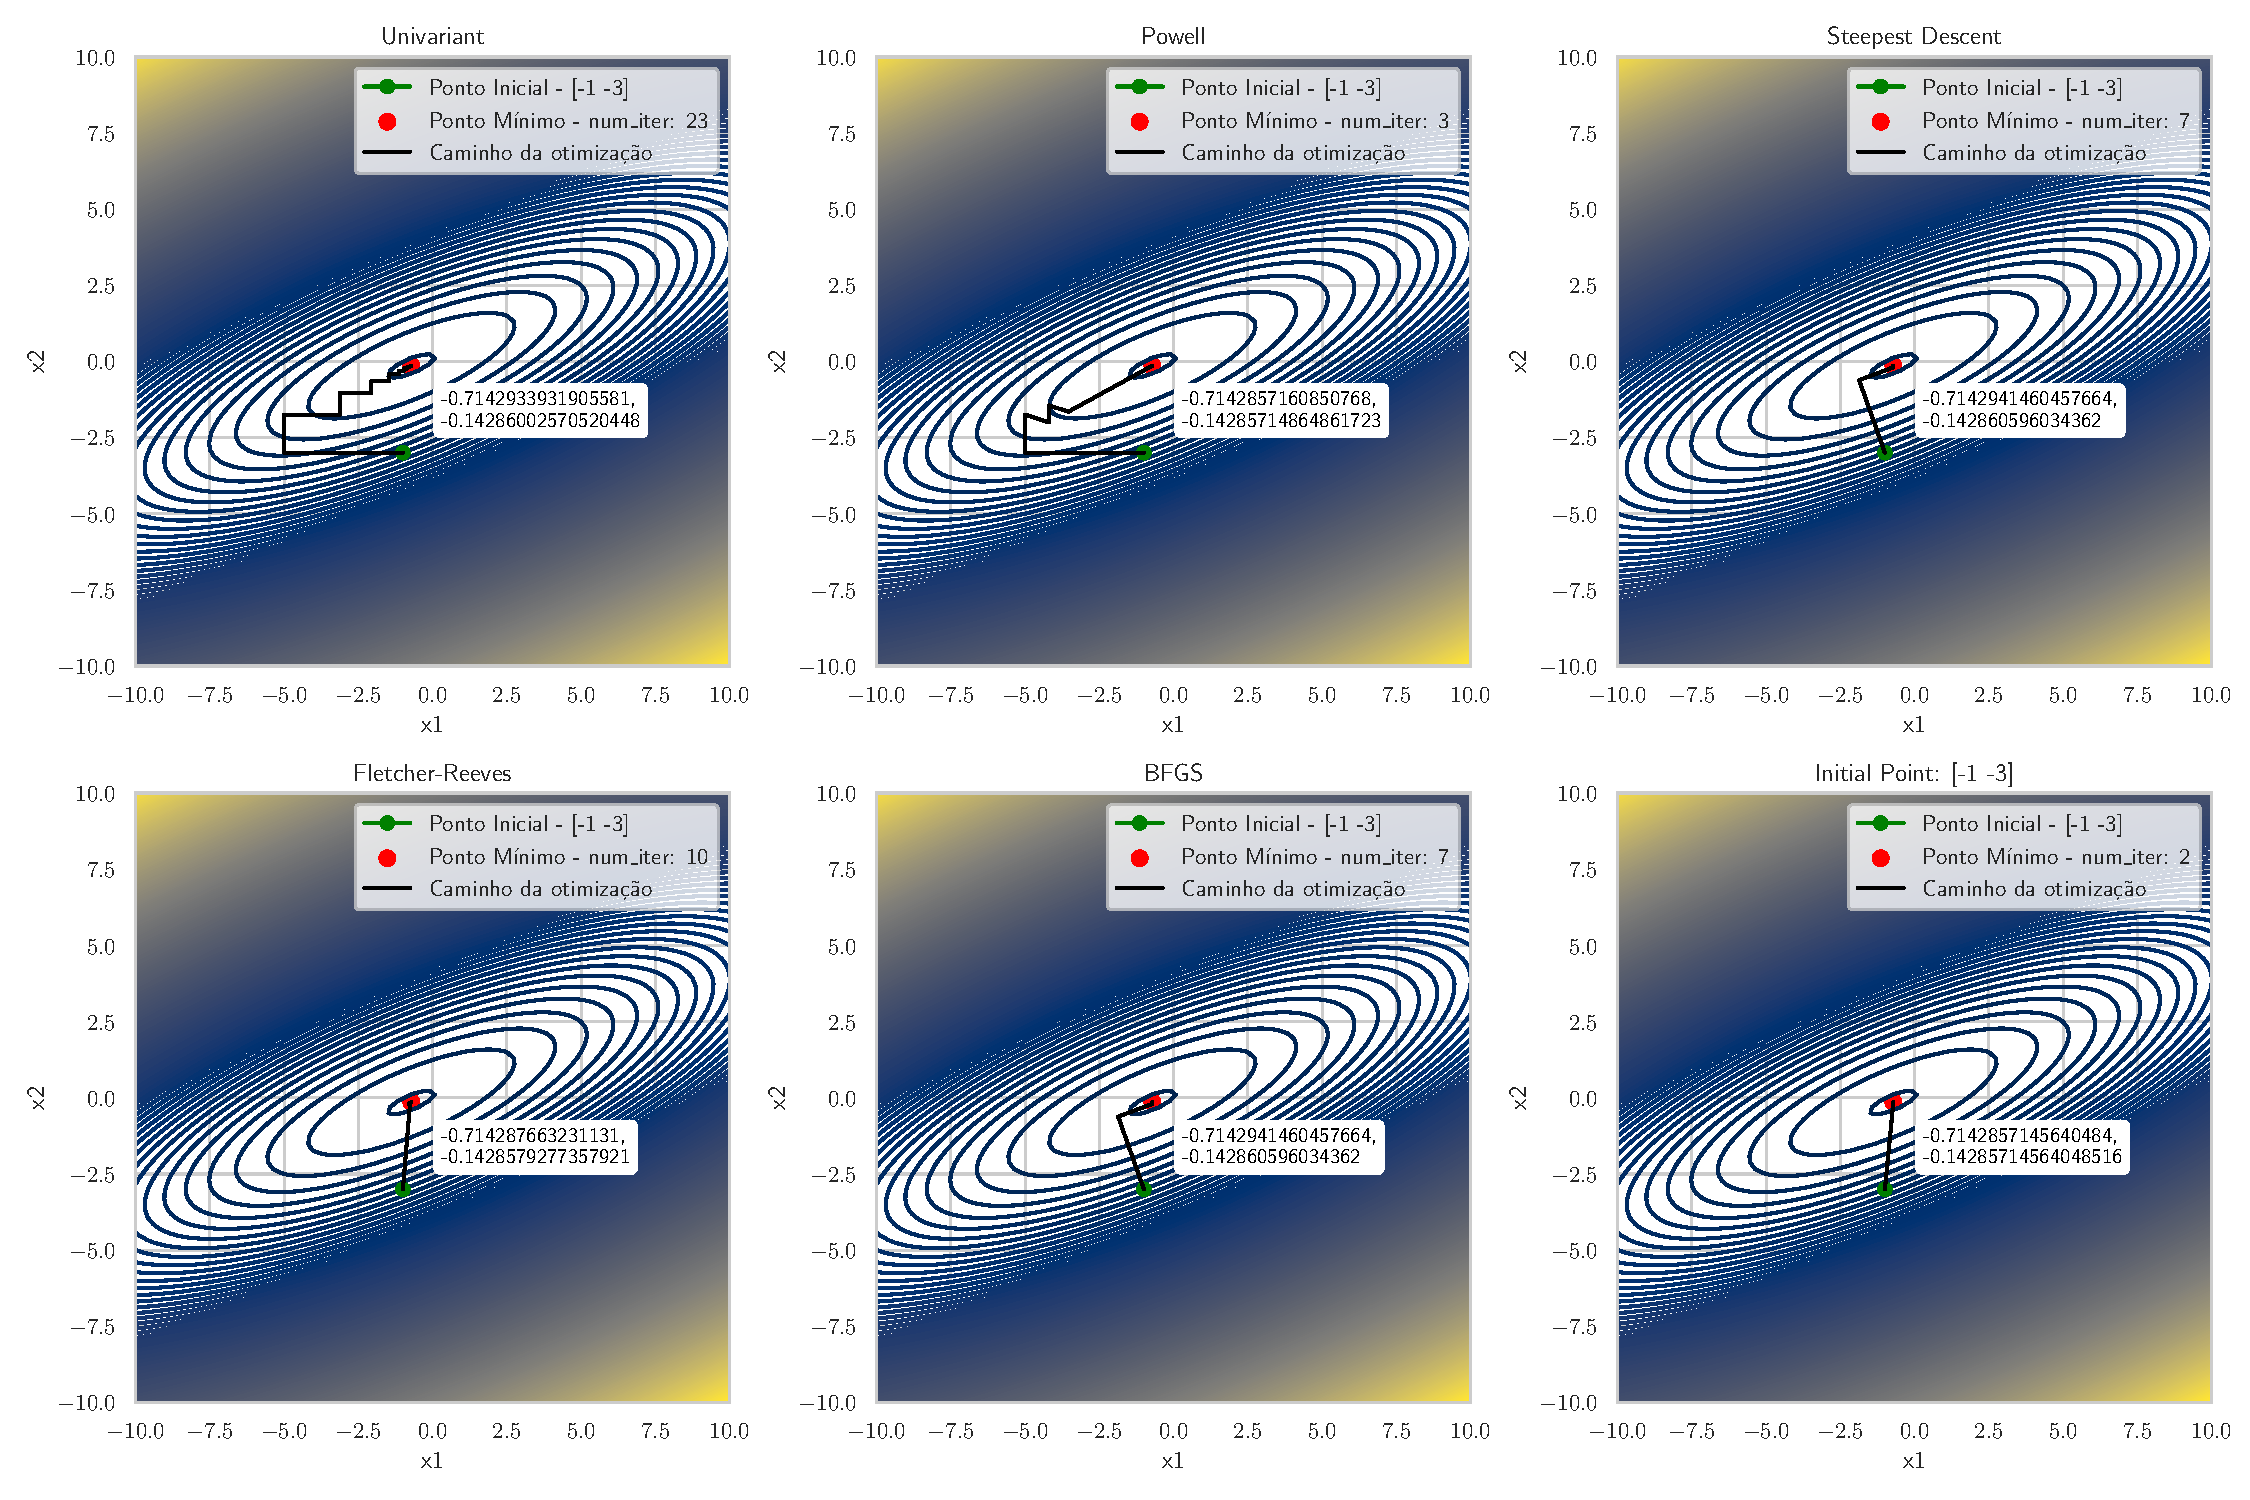
\includegraphics[scale=0.4]{img/questao_1a_[-1 -3].pdf}
\end{figure}

\begin{table}[H]
  \centering
  \begin{tabular}{lll}
    \hline
    \textbf{Método} & \textbf{Ponto Inicial} & \textbf{Ponto Mínimo} \\\hline
    Univariante & $x_{0} =\{2,2\}^{t}$ & [-0.71427, -0.14285]\\
     & $x_{0}=\{-1,-3\}^{t}$ & [-0.71427, -0.14285] \\\hline 
    Powell & $x_{0} =\{2,2\}^{t}$ & [-0.71427, -0.14285]\\
     & $x_{0}=\{-1,-3\}^{t}$ & [-0.71427, -0.14285] \\\hline 
    Steepest Descent & $x_{0} =\{2,2\}^{t}$ & [-0.71427, -0.14285] \\
     & $x_{0}=\{-1,-3\}^{t}$ & [-0.71427, -0.14285] \\\hline 
    Fletcher Reeves & $x_{0} =\{2,2\}^{t}$ & [-0.71427, -0.14285] \\
     & $x_{0}=\{-1,-3\}^{t}$ & [-0.71427, -0.14285] \\\hline 
    BFGS & $x_{0} =\{2,2\}^{t}$ & [-0.71427, -0.14285] \\
     & $x_{0}=\{-1,-3\}^{t}$ & [-0.71427, -0.14285] \\\hline 
    Newton-Rapson & $x_{0} =\{2,2\}^{t}$ & [-0.71427, -0.14285] \\
     & $x_{0}=\{-1,-3\}^{t}$ & [-0.71427, -0.14285] \\\hline 
  \end{tabular}
\end{table}

\paragraph*{Letra (b)}

\begin{equation}
  f(x_{1}, x{2}) = (1+a-bx_{1}-bx_{2})^{2}+(b+x_{1}+ax_{2}-bx_{1}x_{2})^{2}
\end{equation}

\noindent com $a=10$, $b=1$;  $x_{0}=\{10,2\}^{t}$ e $x_{0}=\{-2,-3\}^{t}$

\begin{figure}[H]
  \centering
  \caption{Ponto Inicial: [-2, -3]}
  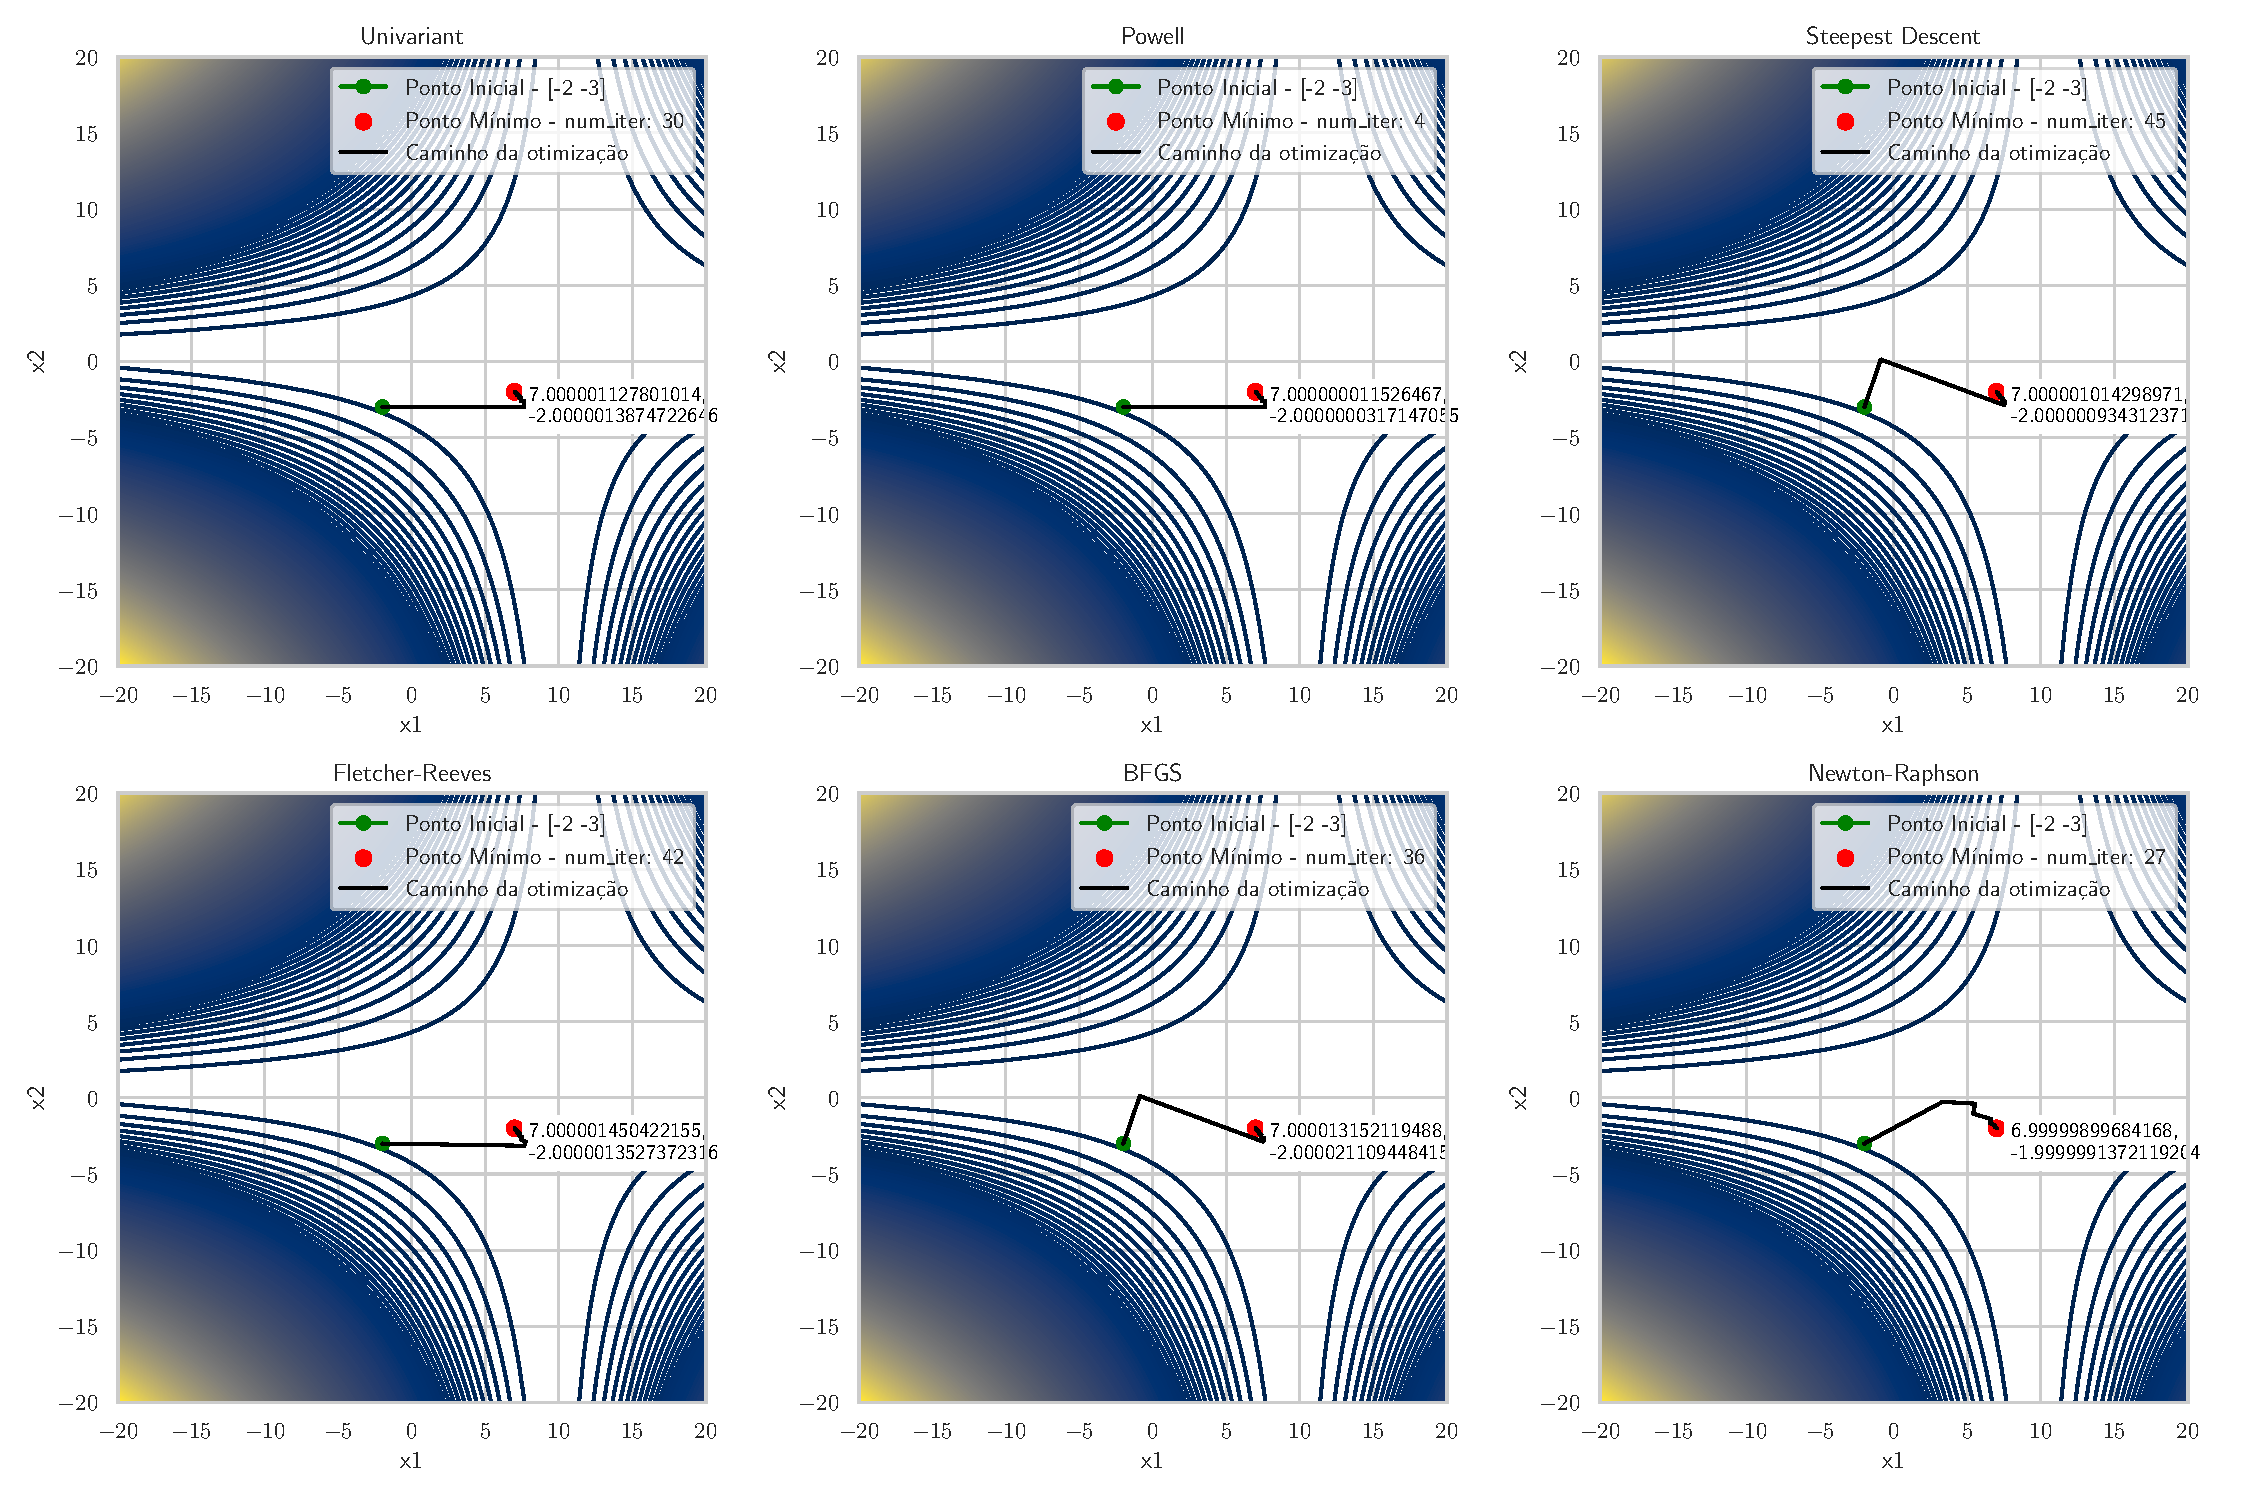
\includegraphics[scale=0.4]{img/questao_1b_[-2 -3].pdf}
\end{figure}

\begin{figure}[H]
  \centering
  \caption{Ponto Inicial: [10, 2]}
  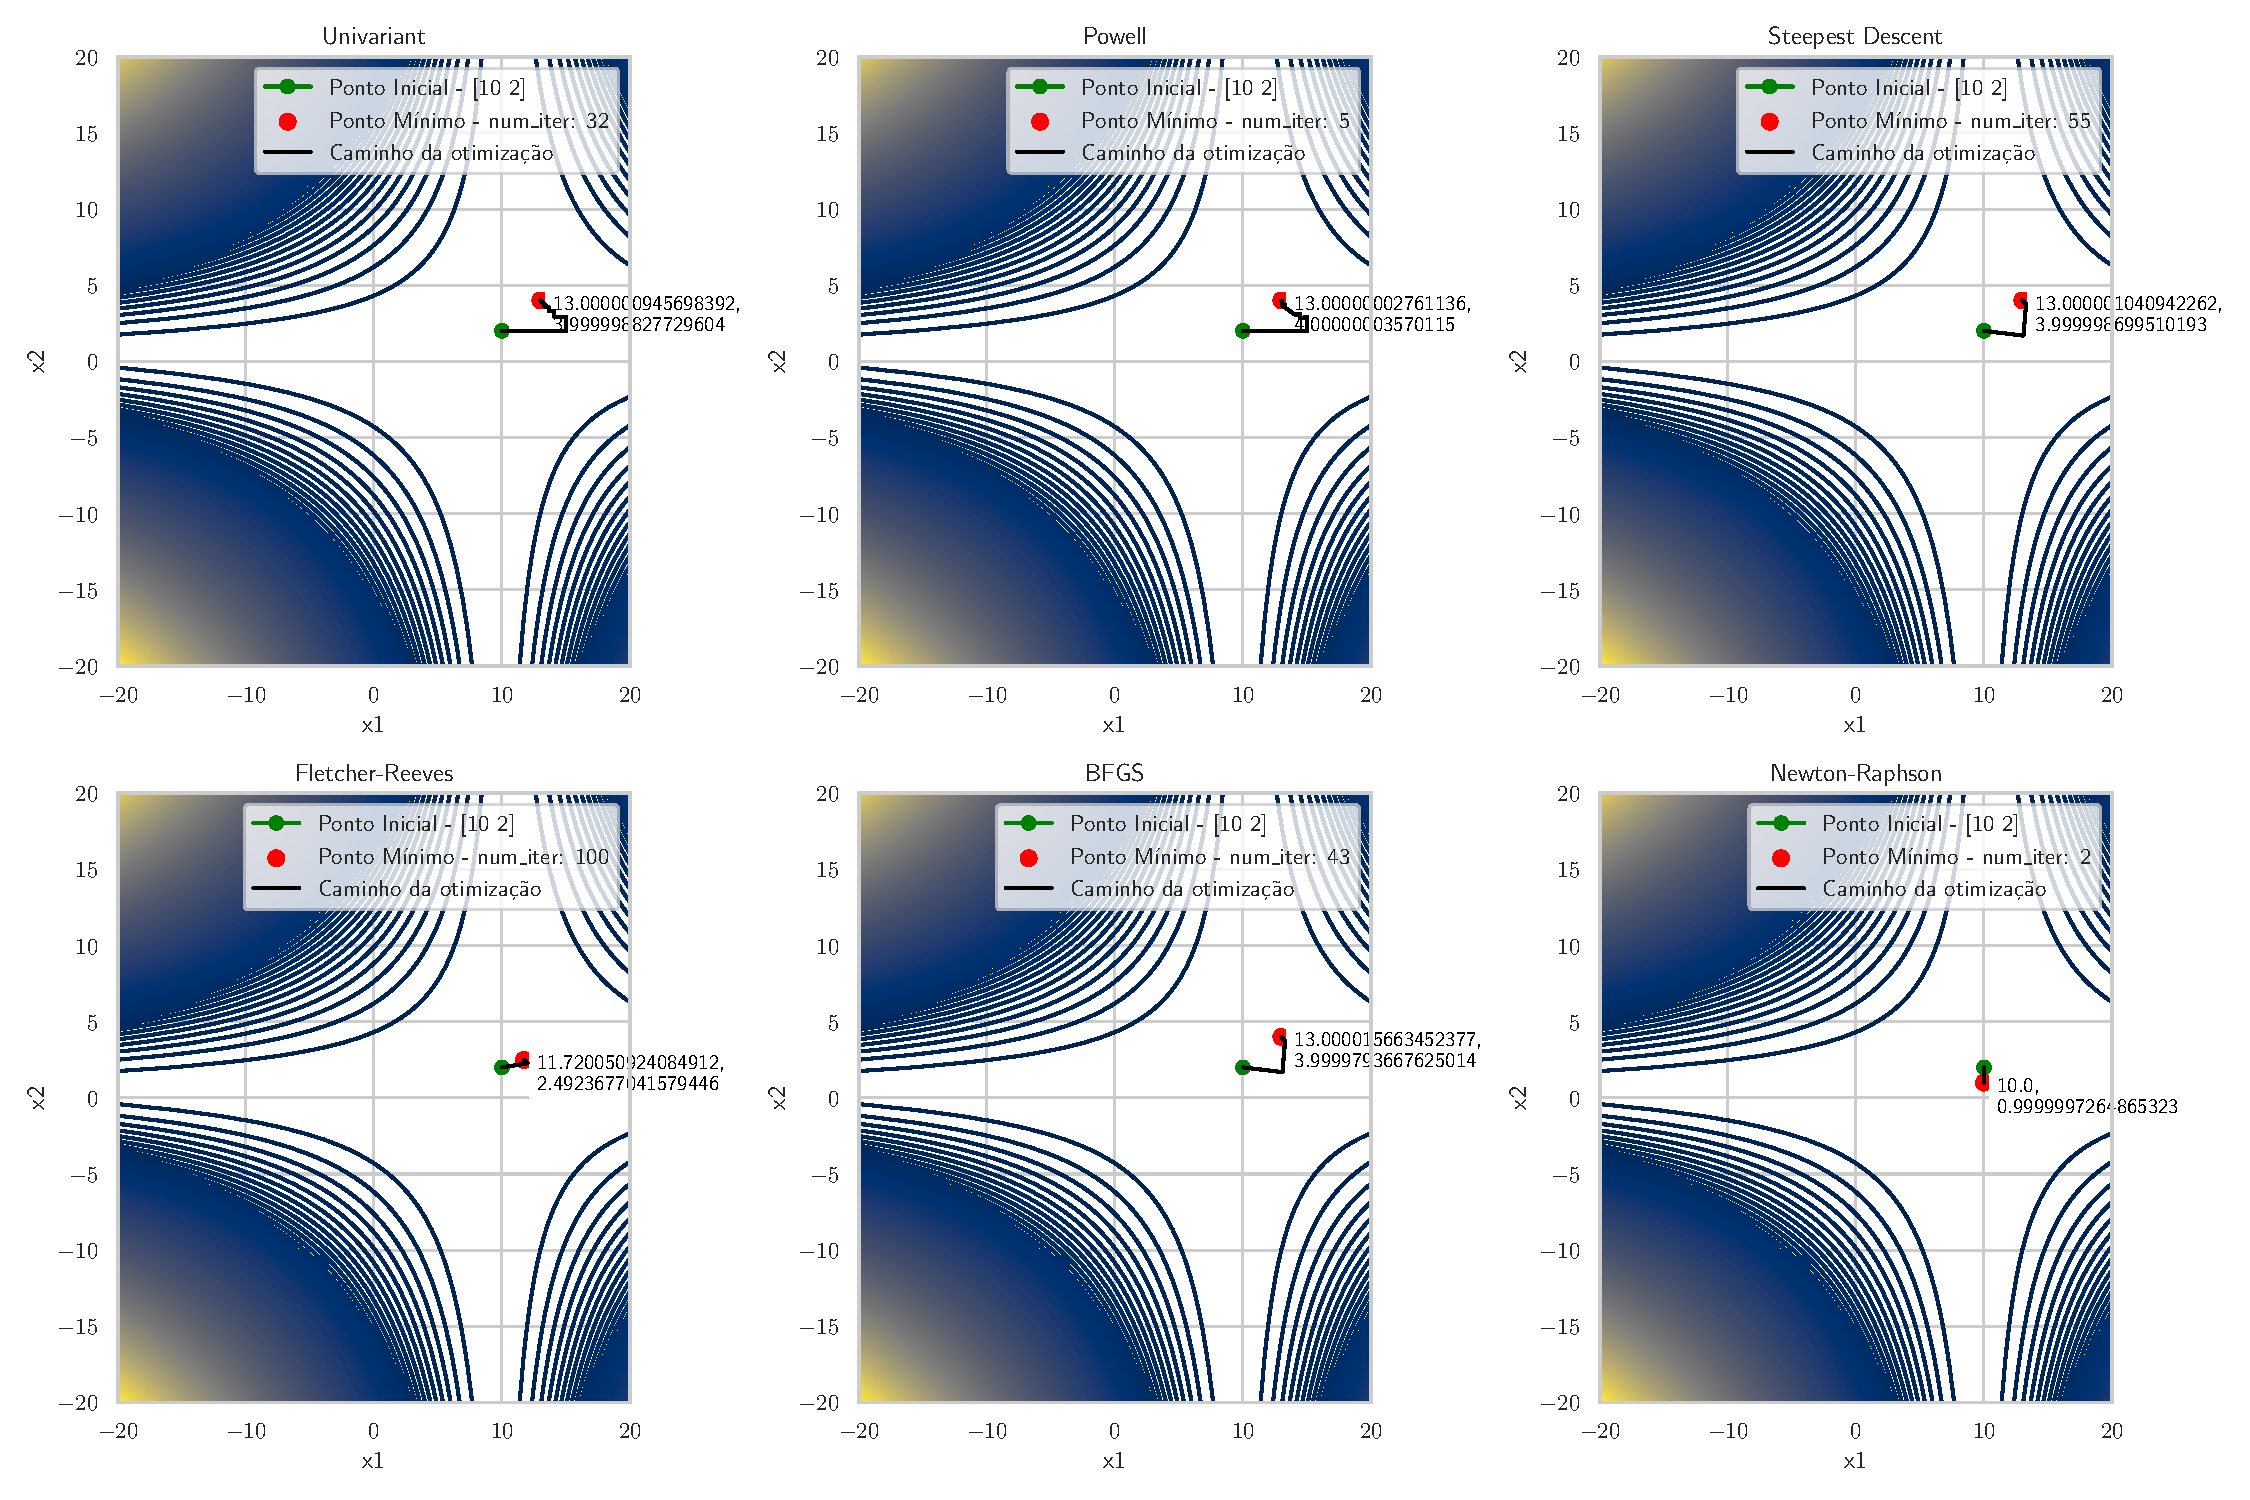
\includegraphics[scale=0.4]{img/questao_1b_2.pdf}
\end{figure}

\begin{table}[H]
  \centering
  \begin{tabular}{lll}
    \hline
    \textbf{Método} & \textbf{Ponto Inicial} & \textbf{Ponto Mínimo} \\\hline
    Univariante & $x_{0} =\{10,2\}^{t}$ & [13.0000, 3.9999]\\
     & $x_{0}=\{-2,-3\}^{t}$ & [7.0000, -2.0000] \\\hline 
    Powell & $x_{0} =\{10,2\}^{t}$ & [13.0000, 3.9999] \\
     & $x_{0}=\{-2,-3\}^{t}$ & [7.0000, -2.0000] \\\hline 
    Steepest Descent & $x_{0} =\{10,2\}^{t}$ & [13.0000, 3.9999] \\
     & $x_{0}=\{-2,-3\}^{t}$ & [7.0000, -2.0000] \\\hline 
  Fletcher Reeves & $x_{0} =\{10,2\}^{t}$ & [11.72005, 2.49236]\\
     & $x_{0}=\{-2,-3\}^{t}$ & [7.0000, -2.0000] \\\hline 
    BFGS & $x_{0} =\{10,2\}^{t}$ & \\
     & $x_{0}=\{-2,-3\}^{t}$ & [7.0000, -2.0000] \\\hline 
    Newton-Rapson & $x_{0} =\{10,2\}^{t}$ & [10, 0.9999]\\
     & $x_{0}=\{-2,-3\}^{t}$ & [6.9999, -1.9999]\\\hline 
  \end{tabular}
\end{table}


\section*{Questão 2} 

\subsection*{Introdução}

$$f(u, v) = \frac{1}{2}\frac{EA_{1}}{L_{1}}(\sqrt{(L_{1}+u)^{2}+v^{2}}-L_{1})^{2}+\frac{1}{2}\frac{EA_{2}}{L_{2}}(\sqrt{(L_{2}+u)^{2}+v^{2}}-L_{2})^{2}-P_{1}v$$

\noindent com os parâmetros $L_{1}=12, L_{2}=8, EA_{1}=12, EA_{2}=80$

A função a ser minimizada é dada por:

$$f(u,v) = (0.5\times(\sqrt{(12+x_{1})^2+x_{2}^2)-12)^2}+(0.5\times10\times(\sqrt{8+x1)^2+x_{2}^2)-8}^2-7\times x_{2})$$

\subsection*{Resultados e discussão}

\begin{figure}[H]
  \centering
  \caption{Ponto Inicial: [9, -2]}
  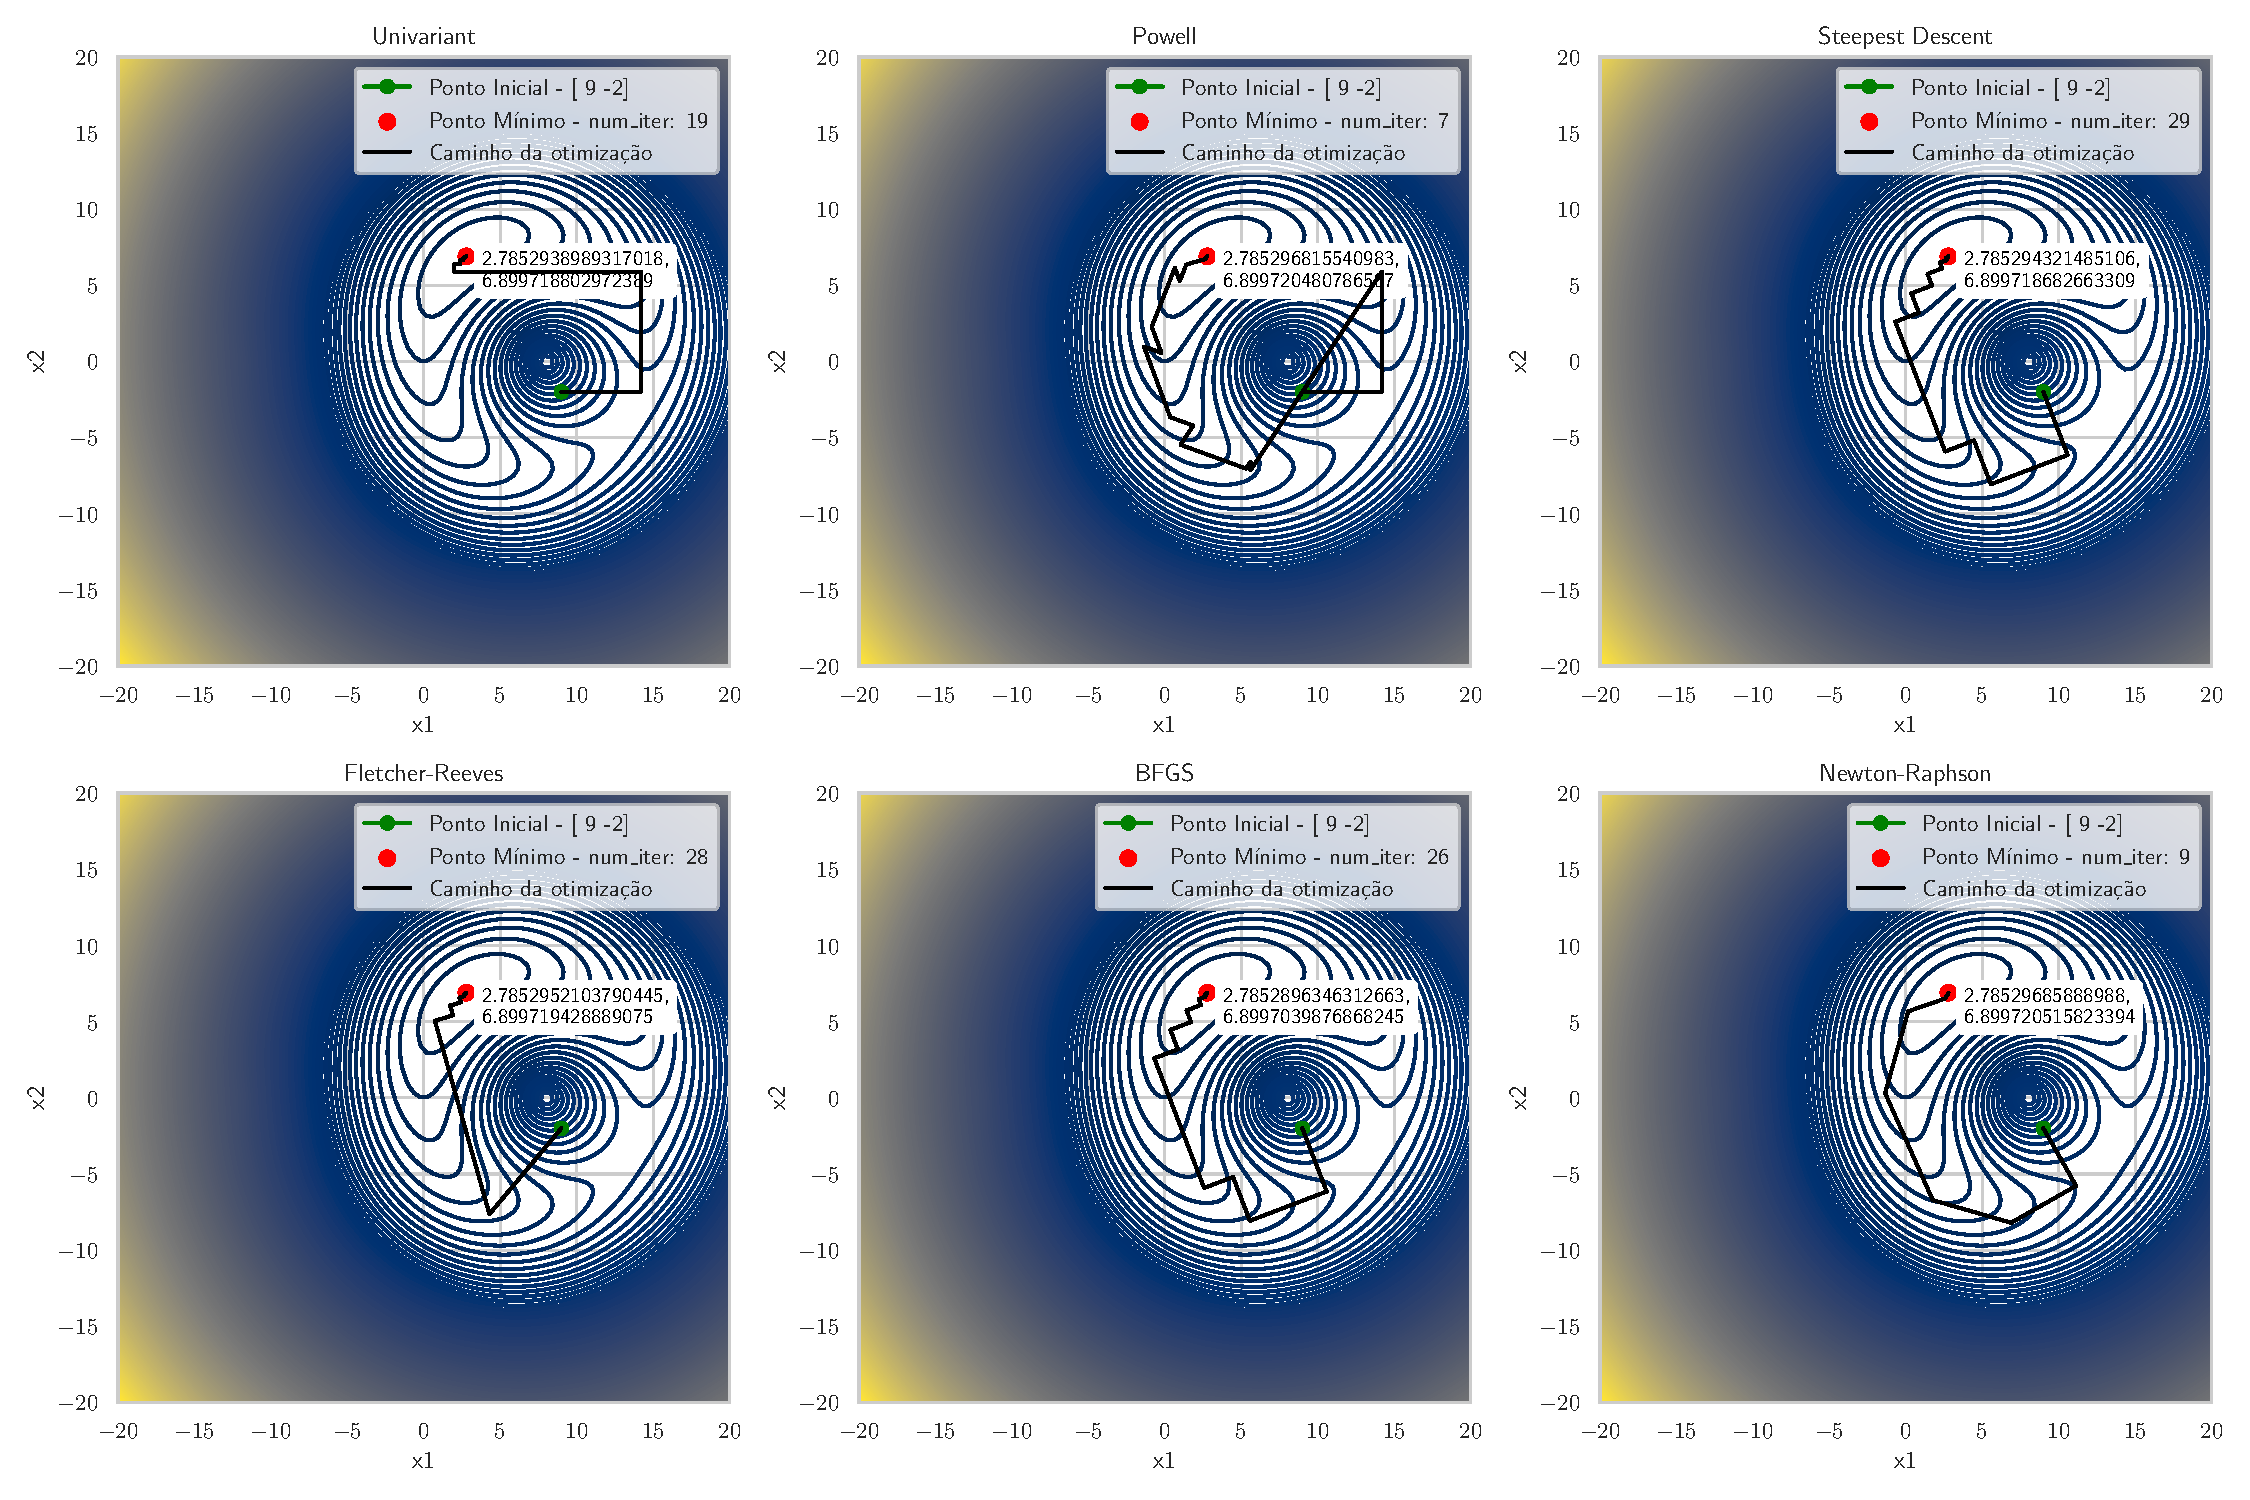
\includegraphics[scale=0.4]{img/questao_2_[ 9 -2].pdf}
\end{figure}

\begin{figure}[H]
  \centering
  \caption{Ponto Inicial: [15, 12]}
  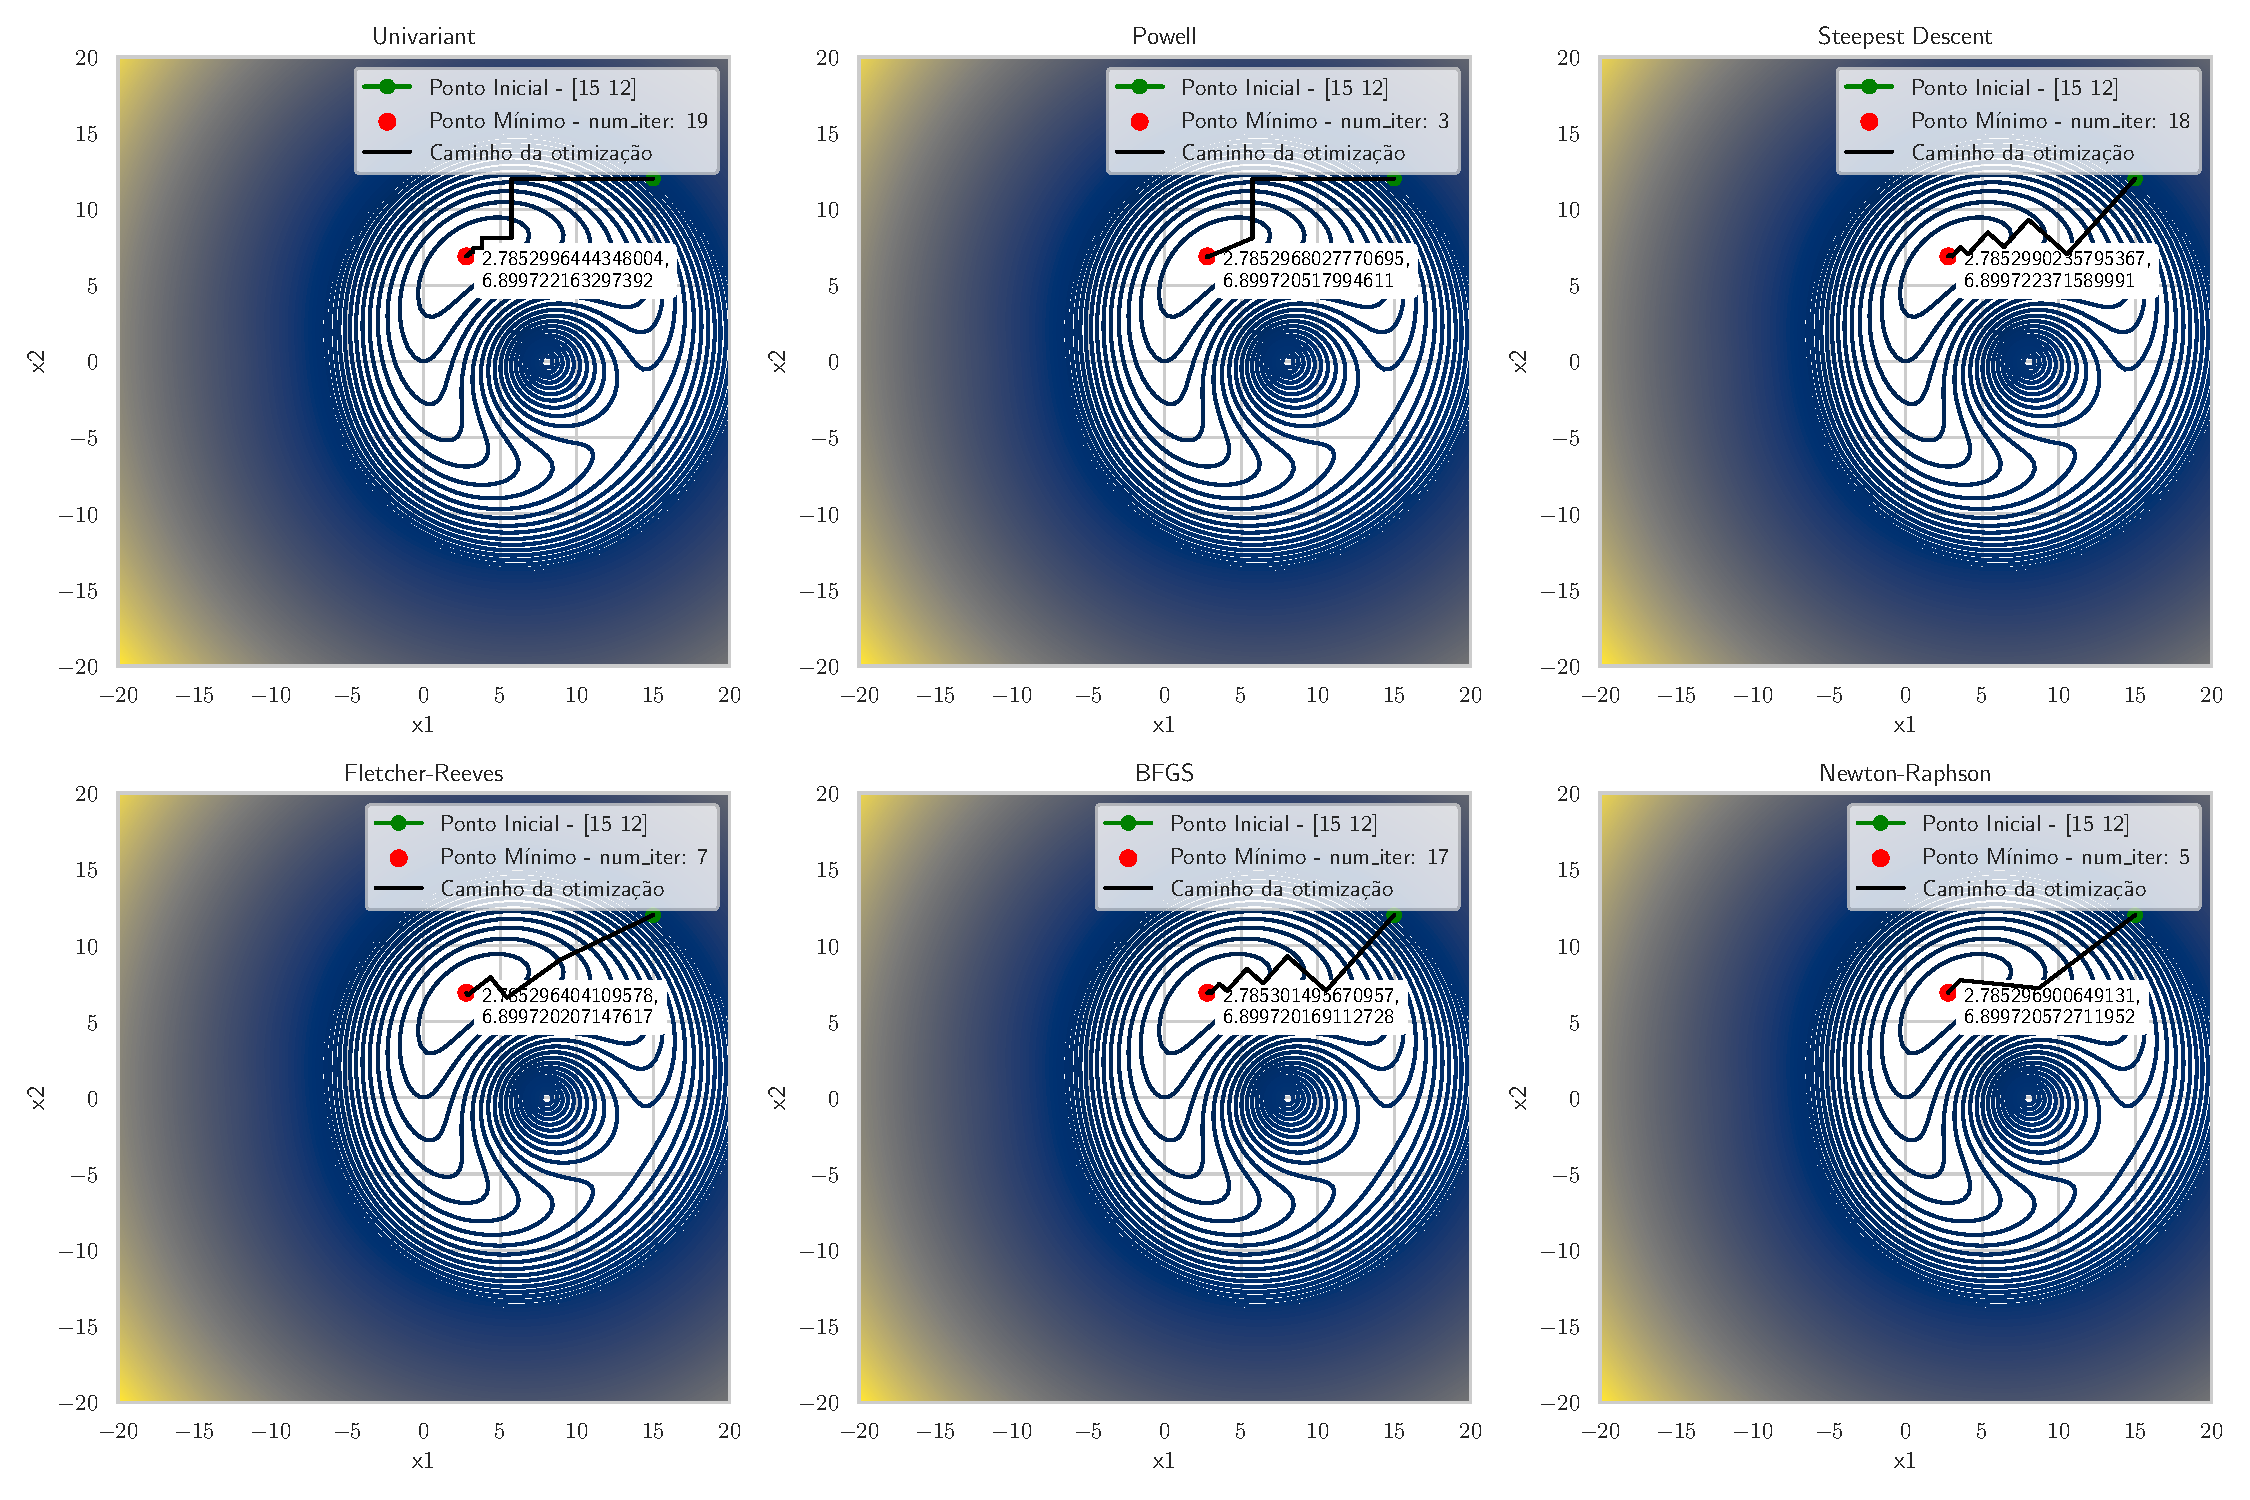
\includegraphics[scale=0.4]{img/questao_2_[15 12].pdf}
\end{figure}

A tabela apresenta resultados obtidos por diferentes métodos de otimização aplicados a um problema específico. Cada linha corresponde a um método de otimização, indicando o ponto inicial, a solução ótima ($xopt$), o valor mínimo da função objetivo ($fmin$), o número de passos necessários para a convergência (\# Passos) e o tempo de execução (Tempo).

\begin{table}[H]
\begin{tabular}{lccccc}
  \hline
  \textbf{Método} & \textbf{Ponto Inicial} & \textbf{xopt} & \textbf{fmin} & \textbf{\# Passos} & \textbf{Tempo} \\
  \hline
  Univariant & [15 12] & [2.78529964 6.89972216] & -36.880428 & 19 & 0.000003 \\
  Powell & [15 12] & [2.7852968  6.89972052] & -36.880428 & 3 & 0.000001 \\
  Steepest Descent & [15 12] & [2.78529902 6.89972237] & -36.880428 & 18 & 0.000001 \\
  Fletcher-Reeves & [15 12] & [2.7852964  6.89972021] & -36.880428 & 7 & 0.000001 \\
  BFGS & [15 12] & [2.7853015  6.89972017] & -36.880428 & 17 & 0.000001 \\
  Newton-Raphson & [15 12] & [2.7852969  6.89972057] & -36.880428 & 5 & 0.000001 \\\hline
  Univariant & [ 9 -2] & [2.7852939 6.8997188] & -36.880428 & 19 & 0.000003 \\
  Powell & [ 9 -2] & [2.78529682 6.89972048] & -36.880428 & 7 & 0.000001 \\
  Steepest Descent & [ 9 -2] & [2.78529432 6.89971868] & -36.880428 & 29 & 0.000001 \\
  Fletcher-Reeves & [ 9 -2] & [2.78529521 6.89971943] & -36.880428 & 28 & 0.000000 \\
  BFGS & [ 9 -2] & [2.78528963 6.89970399] & -36.880428 & 26 & 0.000001 \\
  Newton-Raphson & [ 9 -2] & [2.78529686 6.89972052] & -36.880428 & 9 & 0.000001 \\
  \hline
  \end{tabular}
\end{table}

\end{document}
